% =====================================================================
%  Póster — 2do Workshop Internacional de Estadística
%  Universidad Nacional de Colombia, Sede Manizales · 5 y 6 nov 2026
%
%  Dimensiones: 120 cm de alto x 90 cm de ancho.
%  Compilar con XeLaTeX (recomendado) o LuaLaTeX; pdfLaTeX no sirve.
%  En Overleaf: Menu -> Compiler -> XeLaTeX.
%
%  El diseño (colores, fuente, fondo, pestañas) está en workshop-poster.sty.
%  Aquí solo se escribe el contenido.
% =====================================================================
\documentclass[final]{beamer}
\usepackage{workshop-poster}

\begin{document}
\begin{frame}[t]

% ---------------------------------------------------------------------
% Título y autores
% ---------------------------------------------------------------------
\wsPosterHeader
  {El café, no el dólar: qué mueve su precio en pesos}
  {Información de los autores (Tomás Henao Bonilla, Universidad Nacional de Colombia, Manizales, Colombia)}

% ---------------------------------------------------------------------
% Dos columnas de 34.37 cm, como en la plantilla
% ---------------------------------------------------------------------
\begin{columns}[T,onlytextwidth]

% =========================== COLUMNA IZQUIERDA =======================
\begin{column}{34.37cm}

\begin{block}{Resumen}
El café se cotiza en dólares en Nueva York, pero el caficultor colombiano vende en pesos. ¿Qué pesa más en el precio en pesos: el precio internacional o la tasa de cambio (TRM)? Entre 2016 y 2026, el café en dólares se multiplicó por 2.5, mientras que la TRM terminó casi donde comenzó. Como el precio en pesos es es el producto entre el precio en dólares y la TRM, el retorno en pesos es la adición de los retornos en dólares y los retornos de la TRM, luego la varianza se reparte exactamente: el precio internacional explica del 81\% al 88\% de los retornos en pesos. De esto, cubrirse con futuros de café, elimina la mayor parte del riesgo. % si el café baja pierde con la cosecha pero gana con el futuro. si sube, gana con la cosecha pero pierde con el futuro. 
\end{block}

\begin{block}{Materiales y métodos}
Lorem ipsum dolor sit amet, consectetur adipiscing elit, sed do eiusmod
tempor incididunt ut labore et dolore magna aliqua. Se considera el modelo
\begin{equation}
  y_i = \beta_0 + \sum_{j=1}^{p} \beta_j x_{ij} + \varepsilon_i,
  \qquad \varepsilon_i \sim N(0,\sigma^2),
\end{equation}
cuyos parámetros se estiman por mínimos cuadrados. El procedimiento sigue
estos pasos:
\begin{itemize}
  \item Depuración y descripción de los datos.
  \item Ajuste del modelo y validación de supuestos.
  \item Comparación con métodos alternativos.
\end{itemize}
Duis aute irure dolor in reprehenderit in voluptate velit esse cillum dolore
eu fugiat nulla pariatur. Excepteur sint occaecat cupidatat non proident,
sunt in culpa qui officia deserunt mollit anim id est laborum.
\end{block}

\end{column}

% =========================== COLUMNA DERECHA =========================
\begin{column}{34.37cm}

\begin{block}{Resultados y análisis}
Lorem ipsum dolor sit amet, consectetur adipiscing elit, sed do eiusmod
tempor incididunt ut labore et dolore magna aliqua (Figura~\ref{fig:ejemplo}
y Tabla~\ref{tab:ejemplo}).

\begin{figure}
  \centering
  % Reemplace este recuadro por su figura, por ejemplo:
  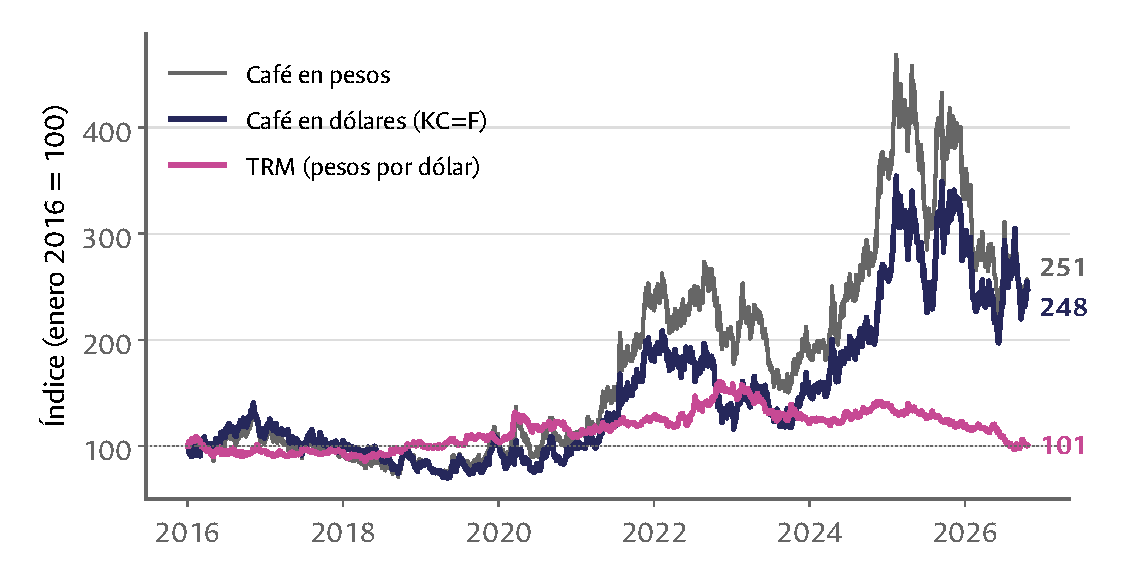
\includegraphics[width=0.9\linewidth]{img/fig_niveles.pdf}
  \caption{Café en dólares, TRM y café en pesos (enero 2016 = 100).}
  \label{fig:ejemplo}
\end{figure}

\begin{figure}
  \centering
  % Reemplace este recuadro por su figura, por ejemplo:
  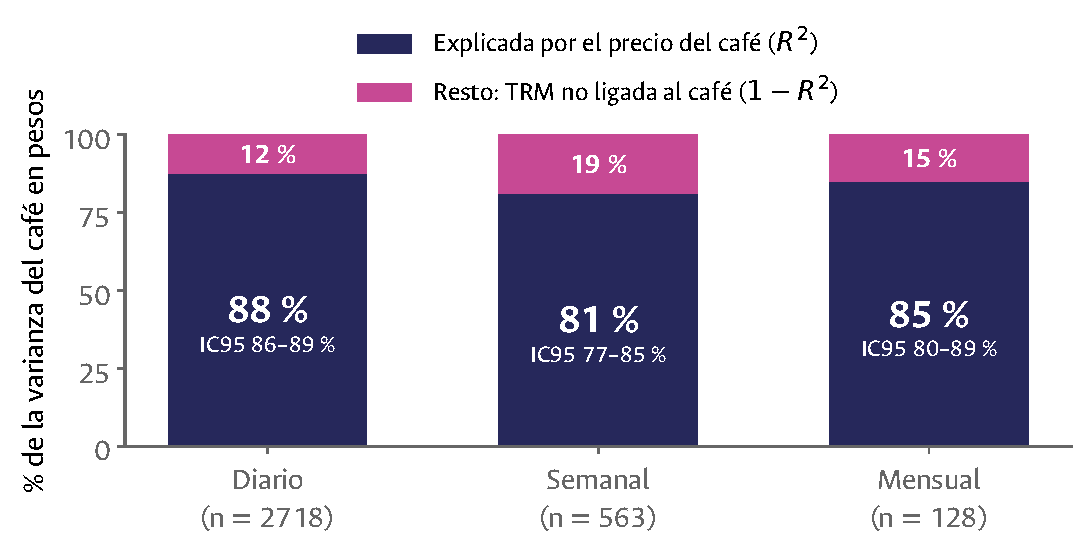
\includegraphics[width=0.9\linewidth]{img/fig_r2.pdf}
  \caption{Reparto de la varianza del retorno del café en pesos, con el IC al 95\% del $R^2$.}
  \label{fig:ejemplo}
\end{figure}

\end{block}

\begin{block}{Conclusiones}
Lorem ipsum dolor sit amet, consectetur adipiscing elit, sed do eiusmod
tempor incididunt ut labore et dolore magna aliqua. Ut enim ad minim veniam,
quis nostrud exercitation ullamco laboris nisi ut aliquip ex ea commodo
consequat.
\end{block}

\begin{block}{Referencias}
\begin{thebibliography}{9}
  \bibitem{ref1} Autor, A. y Autor, B. (2024). Título del artículo.
    \emph{Nombre de la Revista}, 10(2), 1--20.
  \bibitem{ref2} Autor, C. (2022). \emph{Título del libro}. Editorial.
\end{thebibliography}
\end{block}

\end{column}
\end{columns}

\end{frame}
\end{document}
